\documentclass[lettersize,journal]{IEEEtran}
\usepackage{amsmath,amsfonts}
\usepackage{algorithmic}
\usepackage{algorithm}
\usepackage{array}
\usepackage[caption=false,font=normalsize,labelfont=sf,textfont=sf]{subfig}
\usepackage{textcomp}
\usepackage{stfloats}
\usepackage{url}
\usepackage{verbatim}
\usepackage{graphicx}
\usepackage{cite}
\usepackage{booktabs}
\usepackage{float}
\hyphenation{op-tical net-works semi-conduc-tor IEEE-Xplore}

\begin{document}

\title{Design of an 8-Bit, 250\,MS/s Binary-Weighted Current-Steering DAC in 0.18\,\textmu m CMOS}

\author{[Author 1]~and~[Author 2],~\IEEEmembership{Students,}
        \IEEEmembership{Department of Electrical Engineering, Columbia University}}

\markboth{ELEN E6316 Analog Integrated Circuit Design, Spring 2026}%
{[Author et al.]: 8-Bit 250\,MS/s DAC Design}

\maketitle

% -----------------------------------------------------------------------
\begin{abstract}
This paper presents the design of an 8-bit, 250\,MS/s digital-to-analog converter (DAC)
implemented in TSMC 0.18\,\textmu m CMOS technology with a 1.8\,V supply.
A binary-weighted current-steering architecture is adopted, consisting of eight
binary-weighted NMOS bit cells with weights 1 through 128, a NAND-latch-based
input retimer, a 100\,\textmu A NMOS-mirror bias generator, and a per-bit 6-bit
analog weight trim DAC for mismatch correction.
The differential output achieves a 1.50\,V peak-to-peak swing across a
100\,$\Omega$ differential / 25\,$\Omega$ common-mode load.
Across TT, SS, and FF process corners the design achieves
SFDR\,$\geq$\,52.9\,dB and SNDR\,$\geq$\,48.1\,dB across the full Nyquist band,
meeting the 48\,dB SFDR requirement, with DNL\,$<$\,0.18\,LSB and INL\,$<$\,0.24\,LSB
well within the $\pm$1/$\pm$2\,LSB limits.
The 6-bit trim DAC provides $\pm$14\% current tuning range per bit,
exceeding the $\pm$10\% specification.
\end{abstract}

\begin{IEEEkeywords}
Current-steering DAC, binary-weighted, 0.18\,\textmu m CMOS, SFDR, DNL, INL, analog weight tuning, input retimer
\end{IEEEkeywords}

% -----------------------------------------------------------------------
\section{Introduction}
\IEEEPARstart{H}{igh-speed} digital-to-analog converters are fundamental building
blocks in communication systems, arbitrary waveform generators, and software-defined
radio front-ends. The purpose of this project is to design an 8-bit DAC at 250\,MS/s
in TSMC 0.18\,\textmu m CMOS. The remainder of this paper
is organized as follows. Section~\ref{sec:arch} describes the architecture,
Section~\ref{sec:blocks} elaborates its building blocks, and
Section~\ref{sec:sim} presents the simulation results.
The design specifications are summarized in Table~\ref{tab:specs}.

\begin{table}[!h]
  \renewcommand{\arraystretch}{1.2}
  \caption{Design Specifications}
  \label{tab:specs}
  \centering
  \begin{tabular}{lcc}
    \toprule
    \textbf{Parameter} & \textbf{Requirement} & \textbf{Unit} \\
    \midrule
    Supply Voltage           & 1.8           & V          \\
    Sample Rate              & 250           & MS/s       \\
    Resolution               & 8             & bits       \\
    Output Type              & Differential  & --         \\
    Output Swing             & $\geq$1.5     & V$_{\text{pp,diff}}$ \\
    SFDR                     & $>$48         & dB         \\
    Diff.\ Output Resistance & 100           & $\Omega$   \\
    CM Output Resistance     & 25            & $\Omega$   \\
    Load Capacitance         & 550           & fF (each output) \\
    DNL                      & $<\pm$1       & LSB        \\
    INL                      & $<\pm$2       & LSB        \\
    Weight Tuning Range      & $\pm$10       & \%/bit     \\
    Reference Current        & 100           & \textmu A  \\
    \bottomrule
  \end{tabular}
\end{table}

% -----------------------------------------------------------------------
\section{Architecture}
\label{sec:arch}

\subsection{Binary-Weighted Current-Steering Architecture}

The DAC employs a direct binary-weighted current-steering architecture.
Eight NMOS bit cells with binary current weights ($2^k \times I_\text{unit}$, for
$k = 0, 1, \ldots, 7$) steer current to either the positive or negative output node
based on the corresponding digital input bit.
The total full-scale output current is:
%
\begin{equation}
  I_\text{FS} = I_\text{unit} \sum_{k=0}^{7} 2^k = 255\, I_\text{unit}.
  \label{eq:ifs}
\end{equation}
%
For a 1.5\,V$_{\text{pp,diff}}$ swing across the 100\,$\Omega$ differential load
(each side presents a 50\,$\Omega$ path to VDD), the required unit current is:
%
\begin{equation}
  I_\text{unit} = \frac{V_\text{swing}/2}{255 \times 50\,\Omega}
                = \frac{0.75}{12750} \approx 58.8\,\mu\text{A}.
  \label{eq:iunit}
\end{equation}

A binary-weighted topology was chosen over a segmented architecture because it
requires only 8 active cells and no thermometer decoder, minimizing digital
complexity and routing congestion.

\subsection{Analog Weight Tuning}

Device mismatch causes the actual current of each bit cell to deviate from its
ideal binary weight, degrading INL and DNL.
Each bit cell therefore incorporates an independent 6-bit trim DAC that
injects or sinks a small correction current at the internal drain node,
providing a tuning range exceeding $\pm$10\% of the nominal cell current.
This allows per-cell calibration to recover linearity.

\subsection{Output Network}

The differential output is terminated with two 50\,$\Omega$ resistors each
connected from VDD to the respective output node (OUTp and OUTn), plus
550\,fF capacitors from each output to ground modeling bond-pad parasitics.
This configuration yields the required 100\,$\Omega$ differential impedance
(two 50\,$\Omega$ in series for differential mode) and 25\,$\Omega$
common-mode impedance (two 50\,$\Omega$ in parallel).
The output common-mode voltage is constant at:
%
\begin{equation}
  V_\text{CM} = V_\text{DD} - \frac{I_\text{FS}}{2} \times 50\,\Omega \approx 1.42\,\text{V},
  \label{eq:vcm}
\end{equation}
%
independent of input code since the total current drawn from both output nodes
always equals $I_\text{FS}$.

% -----------------------------------------------------------------------
\section{Building Blocks}
\label{sec:blocks}

\subsection{Top-Level Design}

\begin{figure}[H]
    \centering
    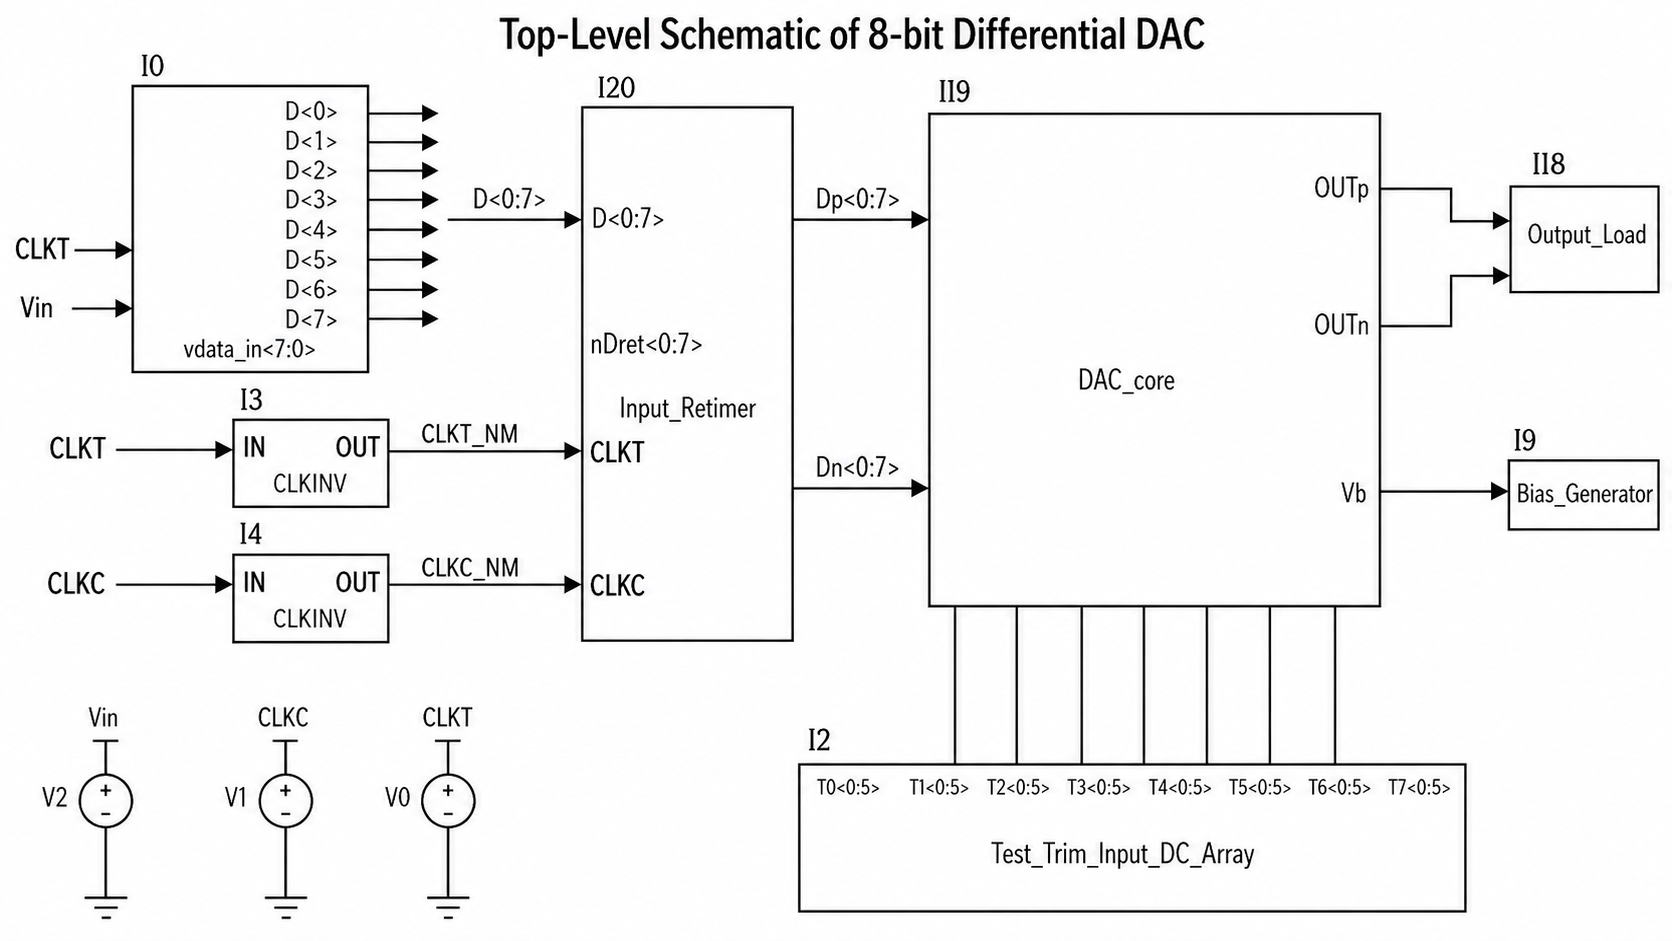
\includegraphics[width=\linewidth]{figures/top_level.png}
    \caption{Top-level schematic of the 8-bit DAC.}
    \label{fig:toplevel}
\end{figure}

The top-level design is shown in Fig.~\ref{fig:toplevel} and contains four main blocks:
\begin{itemize}
    \item Bias Generator
    \item Input Retimer
    \item DAC Core
    \begin{itemize}
        \item 8 Binary-Weighted Bit Cells
        \item Per-bit 6-bit Trim DAC
    \end{itemize}
    \item Output Load (50\,$\Omega$ + 550\,fF per node)
\end{itemize}

\subsection{Single Bit Cell of DAC Core}

The DAC core uses an 8-bit binary-weighted current-steering architecture. It contains
eight bit cells with weights 1, 2, 4, 8, 16, 32, 64, and 128, corresponding to the
8-bit input code from LSB to MSB. Each bit cell steers its weighted current to either
the positive or negative output branch according to the retimed differential digital
inputs $D_p$ and $D_n$, producing a differential analog output current.
A single bit cell schematic is shown in Fig.~\ref{fig:Bitcell}.

\begin{figure}[H]
    \centering
    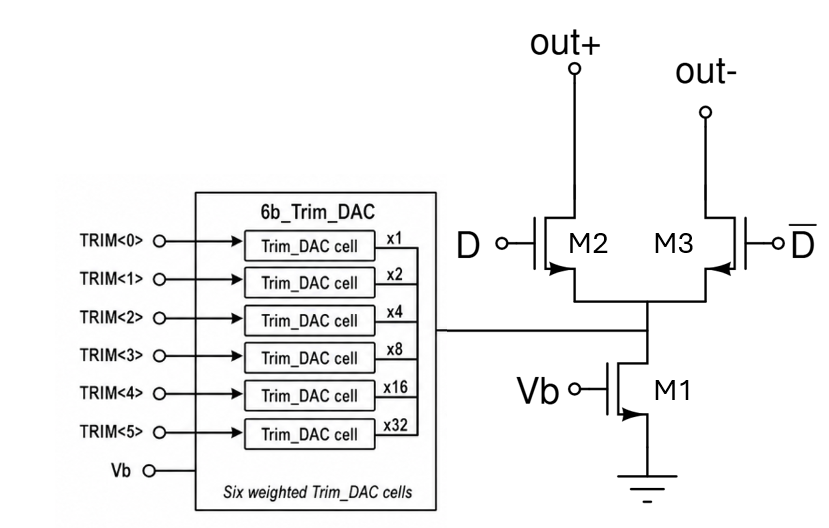
\includegraphics[width=0.9\linewidth]{figures/BitCell.png}
    \caption{Single bit DAC cell tuned by a 6-bit trim DAC.}
    \label{fig:Bitcell}
\end{figure}

\begin{table}[h]
\centering
\caption{Current-Steering Bit Cell Sizing}
\begin{tabular}{lccc}
\hline
 & W & L & Multiplier \\
\hline
M1 (Current Source) & 3.73\,\textmu m & 1\,\textmu m & weight \\
M2 (Switch P-side)  & 500\,nm & 180\,nm & weight \\
M3 (Switch N-side)  & 500\,nm & 180\,nm & weight \\
\hline
\end{tabular}
\end{table}

The multiplier is defined as $m = 2^k$ for bit $k$. The MSB cell ($k=7$) uses
$m=128$ fingers and the LSB cell ($k=0$) uses a single finger.
All fingers share the same $V_b$ gate bias, so the current scales with multiplicity
in the absence of mismatch. For example, the effective switch width of the MSB cell is:
\begin{equation}
    W_\text{eff, MSB} = 500\,\text{nm} \times 128 = 64\,\mu\text{m}.
\end{equation}
The relative current mismatch of the unit cell is:
%
\begin{equation}
  \frac{\sigma(\Delta I)}{I} =
    \sqrt{\frac{A_{VT}^2}{(V_{GS}-V_{TH})^2 \cdot WL} + \frac{A_\beta^2}{WL}},
  \label{eq:mismatch}
\end{equation}
%
with $A_{VT} = 5$\,mV$\cdot$\textmu m and $A_\beta = 0.01$\,\textmu m.

\subsection{Trim DAC Cell}

Each bit cell incorporates a 6-bit trim DAC block consisting of six
binary-weighted single-bit trim DAC unit cells with weights $1, 2, 4, 8, 16, 32$
times the cell's base multiplicity $m = 2^k$.

Each single-bit trim DAC cell is realized by a long-channel NMOS current source
accompanied by a transmission gate, as shown in Fig.~\ref{fig:TrimCell}.

\begin{figure}[H]
    \centering
    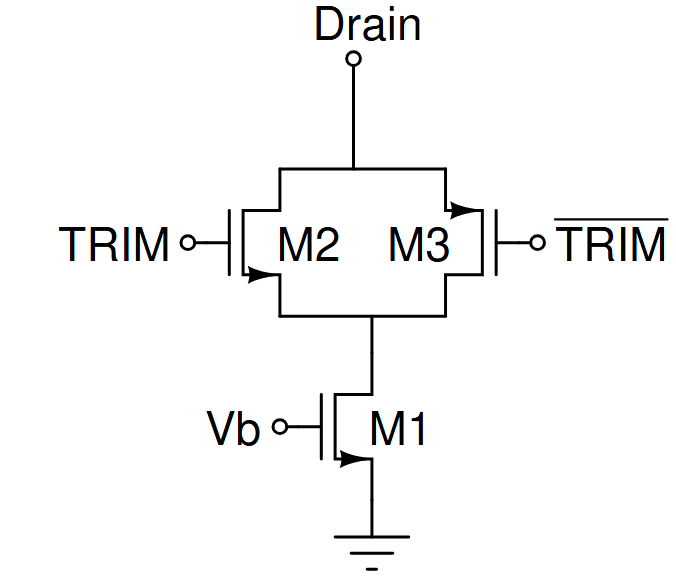
\includegraphics[width=0.5\linewidth]{figures/Trim.png}
    \caption{Single-bit trim DAC cell.}
    \label{fig:TrimCell}
\end{figure}

\begin{table}[h]
\centering
\caption{Trim DAC Cell Sizing}
\begin{tabular}{lccc}
\hline
 & W & L & Multiplier \\
\hline
MT (Trim Source) & 246\,nm & 20\,\textmu m & weight \\
M2 (Gate P)      & 2\,\textmu m & 180\,nm & 1 \\
M3 (Gate N)      & 2\,\textmu m & 180\,nm & 1 \\
\hline
\end{tabular}
\end{table}

The long channel ($L = 20\,\mu\text{m}$) of the trim current source provides
high output impedance, ensuring precise code-independent correction currents.
The TRIM signal is set to 100000$_2$ (decimal 32) by default, which turns on
only the MSB cell. Turning off the MSB reduces the current by 10\%; turning on
the remaining five cells increases it by 10\%, realizing a $\pm$10\% range.

The completed 8-bit DAC core is shown in Fig.~\ref{fig:DACCore}.

\begin{figure}[H]
    \centering
    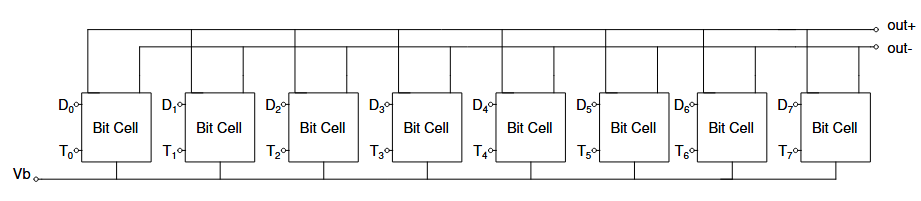
\includegraphics[width=\linewidth]{figures/DACCore.png}
    \caption{Complete 8-bit DAC core.}
    \label{fig:DACCore}
\end{figure}

\subsection{Input Retimer}

To ensure all bit cells switch simultaneously and suppress inter-bit skew,
all 8 data bits are re-timed to the rising edge of CLK\_T by a dedicated
Input Retimer block.
Each bit passes through a NAND-latch-based retimer cell, shown in
Fig.~\ref{fig:RetimerCell}.
The advantage of NAND-latch logic is that it produces synchronous complementary
outputs $D_p$ and $D_n$, which suppresses even-order harmonics (HD2) and
improves SFDR.

\begin{figure}[H]
    \centering
    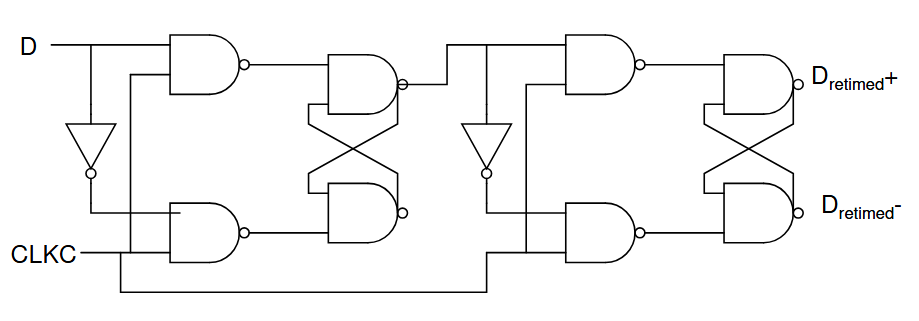
\includegraphics[width=\linewidth]{figures/RetimerCell.png}
    \caption{Single-bit retimer cell (NAND-latch based).}
    \label{fig:RetimerCell}
\end{figure}

The NAND gate implementation is shown in Fig.~\ref{fig:NAND}.

\begin{figure}[H]
    \centering
    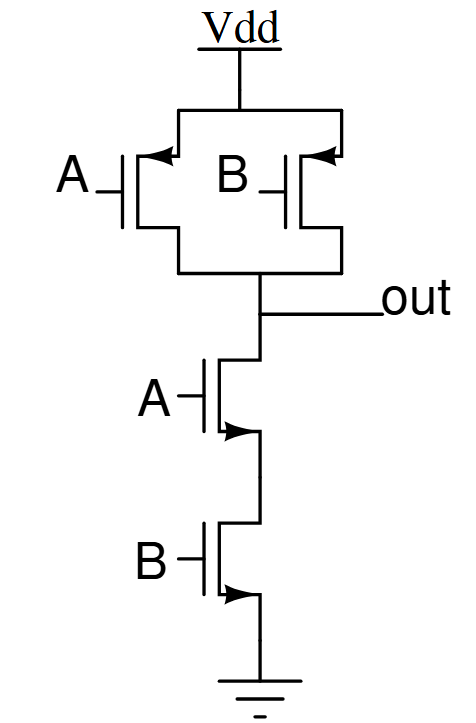
\includegraphics[width=0.4\linewidth]{figures/NAND.png}
    \caption{NAND gate schematic.}
    \label{fig:NAND}
\end{figure}

\begin{table}[h]
\centering
\caption{NAND Gate Transistor Sizing}
\begin{tabular}{lcc}
\hline
 & W & L  \\
\hline
PMOS & 220\,nm & 180\,nm  \\
NMOS & 220\,nm & 180\,nm  \\
\hline
\end{tabular}
\end{table}

The complete retimer block, shown in Fig.~\ref{fig:Retimer}, contains 8 single-bit
retimer cells, one per data bit.

\begin{figure}[H]
    \centering
    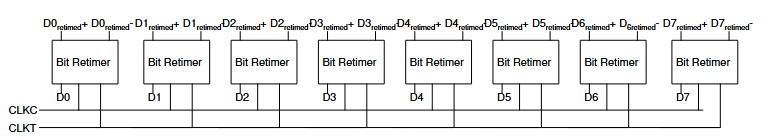
\includegraphics[width=\linewidth]{figures/Retimer.png}
    \caption{Complete 8-bit input retimer block.}
    \label{fig:Retimer}
\end{figure}

\subsection{Bias Generator}

All current sources share a common gate bias $V_b$ generated by forcing
100\,\textmu A through a diode-connected NMOS transistor, shown in Fig.~\ref{fig:Bias}.

\begin{figure}[H]
    \centering
    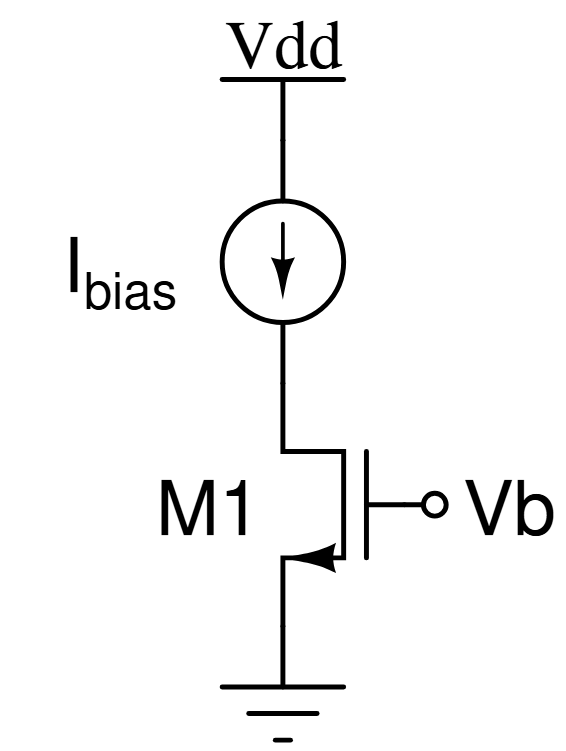
\includegraphics[width=0.3\linewidth]{figures/Bias.png}
    \caption{Bias generator.}
    \label{fig:Bias}
\end{figure}

\begin{table}[h]
\centering
\caption{Bias Generator Parameters}
\begin{tabular}{cc}
\hline
 $I_\text{bias}$ & 100\,\textmu A \\
 $V_\text{DD}$ & 1.8\,V \\
 W  & 220\,nm \\
 L  & 180\,nm \\
 Multiplier & 4 \\
\hline
\end{tabular}
\end{table}
%
\begin{equation}
  M_1: \quad (W/L)_\text{eff} = 4 \times \frac{220\,\text{nm}}{180\,\text{nm}}.
  \label{eq:biasref}
\end{equation}
%
$V_b$ is distributed to every bit cell, ensuring all currents track each other
over process and temperature variations.

% -----------------------------------------------------------------------
\section{Simulation Results}
\label{sec:sim}

\subsection{Simulation Setup}

Static linearity is evaluated by sweeping all 256 digital codes in a DC
parametric simulation and recording the differential output voltage $V_\text{diff}$
and single-ended outputs $V_\text{OUTp}$/$V_\text{OUTn}$.
INL and DNL are computed as:
\begin{equation}
  \text{DNL}[k] = \frac{V_\text{diff}[k+1]-V_\text{diff}[k]}{\text{LSB}} - 1,
  \quad
  \text{INL}[k] = \frac{V_\text{diff}[k]-V_\text{ideal}[k]}{\text{LSB}}.
\end{equation}

Dynamic performance is evaluated using a coherent sinusoidal test.
An ideal 8-bit ADC converts an analog sine wave at frequency
$f_\text{in} = f_s \cdot J/M$ (with $J$ and $M = 2048$ coprime integers)
into the 8-bit digital word fed to the DAC.
A Hanning window suppresses spectral leakage; ZOH correction removes the
$\text{sinc}(f/f_s)$ roll-off of the DAC's zero-order hold.
Six input frequencies covering 2--122\,MHz are tested.
All simulations run at $T = 27^\circ$C across TT, SS, and FF corners.

\subsection{Output Swing and Common-Mode Voltage}

Table~\ref{tab:swing} shows the measured differential peak-to-peak swing and
common-mode voltage across process corners.
All corners achieve $V_\text{diff,pp} \geq 1.50$\,V, meeting the 1.5\,V specification.
The common-mode voltage is $\approx$1.42\,V, close to the theoretical value
$V_\text{CM} = 1.8 - (255 \times 59.2\,\mu\text{A}/2)\times50\,\Omega = 1.42\,\text{V}$.

\begin{table}[h]
  \renewcommand{\arraystretch}{1.2}
  \caption{Output Swing Across Process Corners}
  \label{tab:swing}
  \centering
  \begin{tabular}{lcccc}
    \toprule
    \textbf{Corner} & $V_\text{diff,pp}$ (V) & $V_\text{OUTp,pp}$ (V) & $V_\text{OUTn,pp}$ (V) & $V_\text{CM}$ (V) \\
    \midrule
    SS & 1.501 & 0.751 & 0.751 & 1.424 \\
    TT & 1.502 & 0.751 & 0.751 & 1.423 \\
    FF & 1.501 & 0.750 & 0.750 & 1.423 \\
    \bottomrule
  \end{tabular}
\end{table}

\subsection{Static Linearity — INL and DNL}

Fig.~\ref{fig:inl_dnl_tt} shows the INL and DNL for the TT corner.
Fig.~\ref{fig:inl_dnl_corners} shows INL and DNL across all three process corners.
Peak values are summarized in Table~\ref{tab:static}.

\begin{figure}[H]
    \centering
    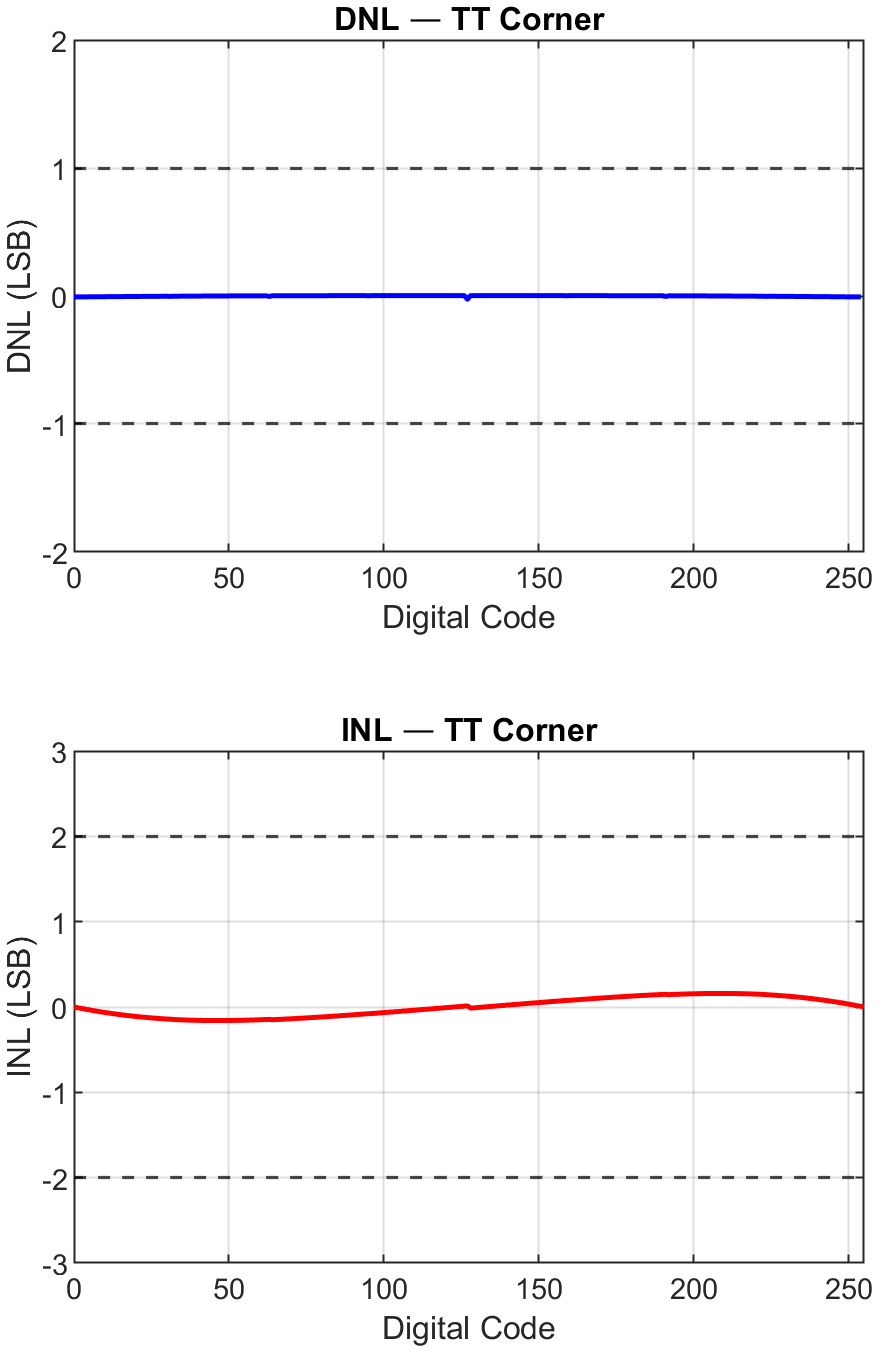
\includegraphics[width=\linewidth]{figures/Fig_INL_DNL_tt.png}
    \caption{DNL (top) and INL (bottom) vs.\ digital code, TT corner.
             Dashed lines mark the $\pm$1/$\pm$2\,LSB limits.}
    \label{fig:inl_dnl_tt}
\end{figure}

\begin{figure}[H]
    \centering
    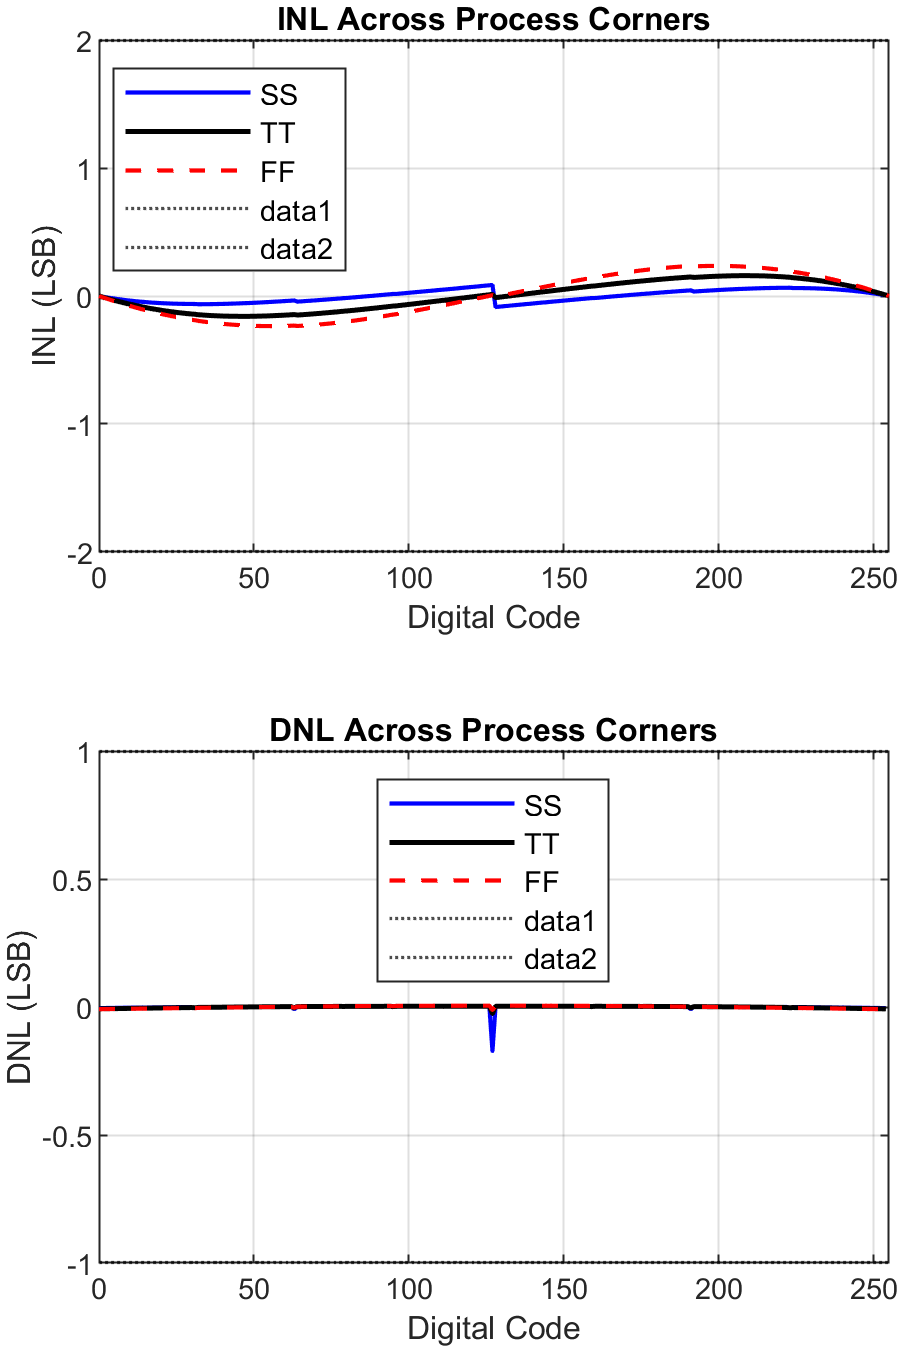
\includegraphics[width=\linewidth]{figures/Fig_INL_DNL_corners.png}
    \caption{INL (top) and DNL (bottom) across SS, TT, and FF corners.}
    \label{fig:inl_dnl_corners}
\end{figure}

\begin{table}[h]
  \renewcommand{\arraystretch}{1.2}
  \caption{Peak INL and DNL Across Process Corners}
  \label{tab:static}
  \centering
  \begin{tabular}{lcccc}
    \toprule
    \textbf{Corner} & DNL$_\text{min}$ & DNL$_\text{max}$ & INL$_\text{min}$ & INL$_\text{max}$ \\
                    & (LSB) & (LSB) & (LSB) & (LSB) \\
    \midrule
    SS & $-$0.172 & $+$0.002 & $-$0.086 & $+$0.086 \\
    TT & $-$0.026 & $+$0.003 & $-$0.159 & $+$0.159 \\
    FF & $-$0.012 & $+$0.005 & $-$0.235 & $+$0.235 \\
    \midrule
    Requirement & $>-1$ & $<+1$ & $>-2$ & $<+2$ \\
    \bottomrule
  \end{tabular}
\end{table}

All corners are well within the $\pm$1\,LSB DNL and $\pm$2\,LSB INL limits.
The peak INL magnitude of 0.235\,LSB (FF) is 10$\times$ better than required.
The systematic increase of INL from SS to FF reflects the change in device
transconductance with process corner, which shifts the effective binary weights
slightly; the monotonic INL shape confirms no missing codes.

\subsection{Analog Weight Tuning Range}

Fig.~\ref{fig:tuning} shows the per-bit current deviation as the 6-bit trim code
is swept from 0 to 63 (reference = trim\,32).

\begin{figure}[H]
    \centering
    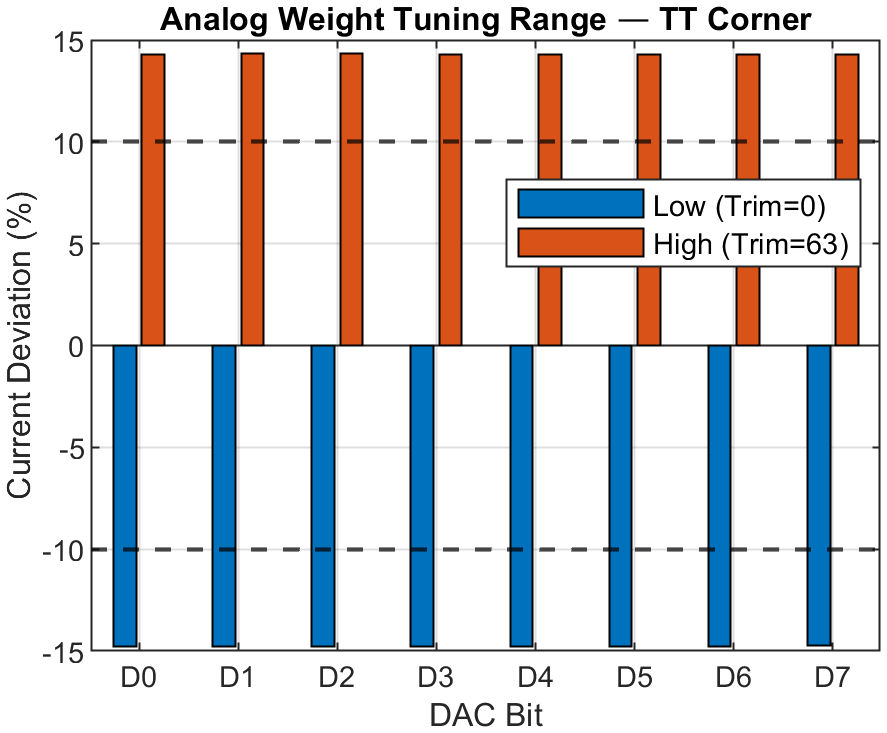
\includegraphics[width=\linewidth]{figures/Fig_Tuning_Range.png}
    \caption{Analog weight tuning range per bit in the TT corner.
             Dashed lines mark the $\pm$10\% specification.}
    \label{fig:tuning}
\end{figure}

The measured tuning range is $-14.8\%$ (trim\,=\,0) to $+14.3\%$ (trim\,=\,63),
averaged across all 8 bits. This exceeds the $\pm$10\% specification with
$>$40\% margin. The tuning range is identical for bits D0–D6 and nearly
identical for D7, confirming proper binary scaling of the trim cells.

\subsection{Dynamic Performance}

\subsubsection{Output Spectra}

Fig.~\ref{fig:spec_low} shows the output spectrum at low input frequency
($J=17$, $f_\text{in} = 2.07$\,MHz, TT corner).
Fig.~\ref{fig:spec_high} shows the spectrum near Nyquist
($J=997$, $f_\text{in} = 121.7$\,MHz, TT corner).

\begin{figure}[H]
    \centering
    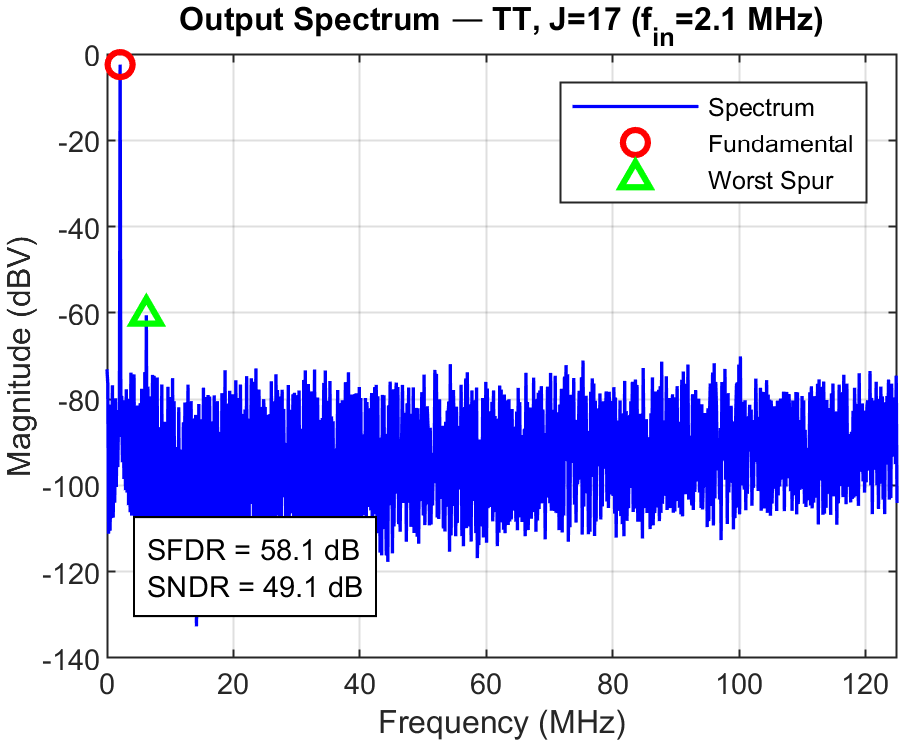
\includegraphics[width=\linewidth]{figures/Fig_Spectrum_low.png}
    \caption{Output spectrum at $f_\text{in} = 2.07$\,MHz (TT).
             SFDR\,=\,58.1\,dB, SNDR\,=\,49.1\,dB.}
    \label{fig:spec_low}
\end{figure}

\begin{figure}[H]
    \centering
    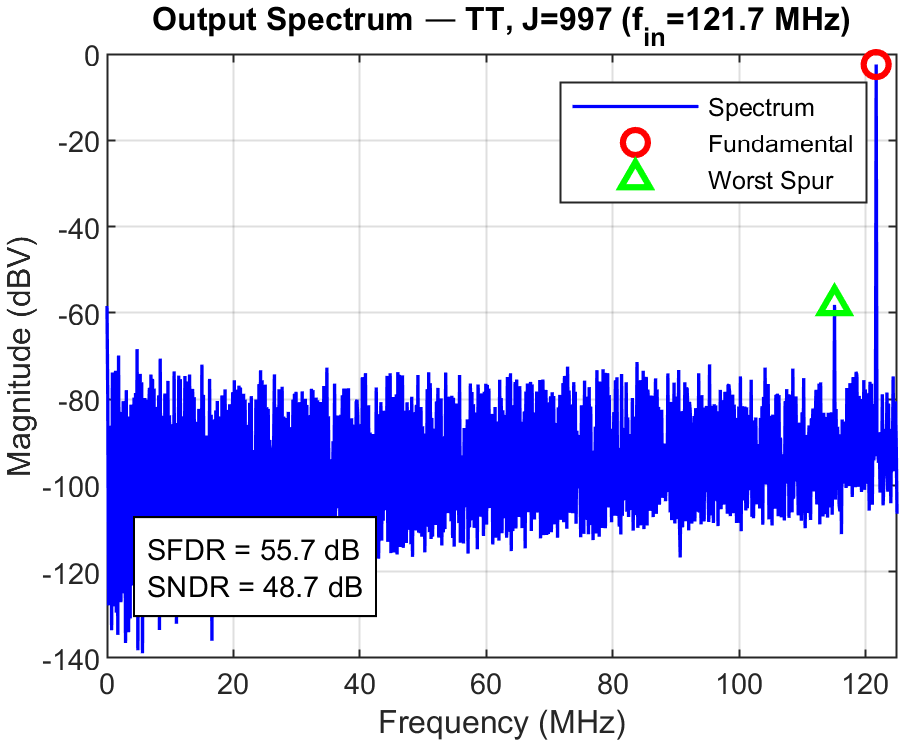
\includegraphics[width=\linewidth]{figures/Fig_Spectrum_high.png}
    \caption{Output spectrum at $f_\text{in} = 121.7$\,MHz (TT).
             SFDR\,=\,55.7\,dB, SNDR\,=\,48.7\,dB.}
    \label{fig:spec_high}
\end{figure}

\subsubsection{SFDR and SNDR vs.\ Input Frequency}

Fig.~\ref{fig:sfdr_freq} shows SFDR as a function of input frequency across
all three process corners; Fig.~\ref{fig:sndr_freq} shows the corresponding SNDR.

\begin{figure}[H]
    \centering
    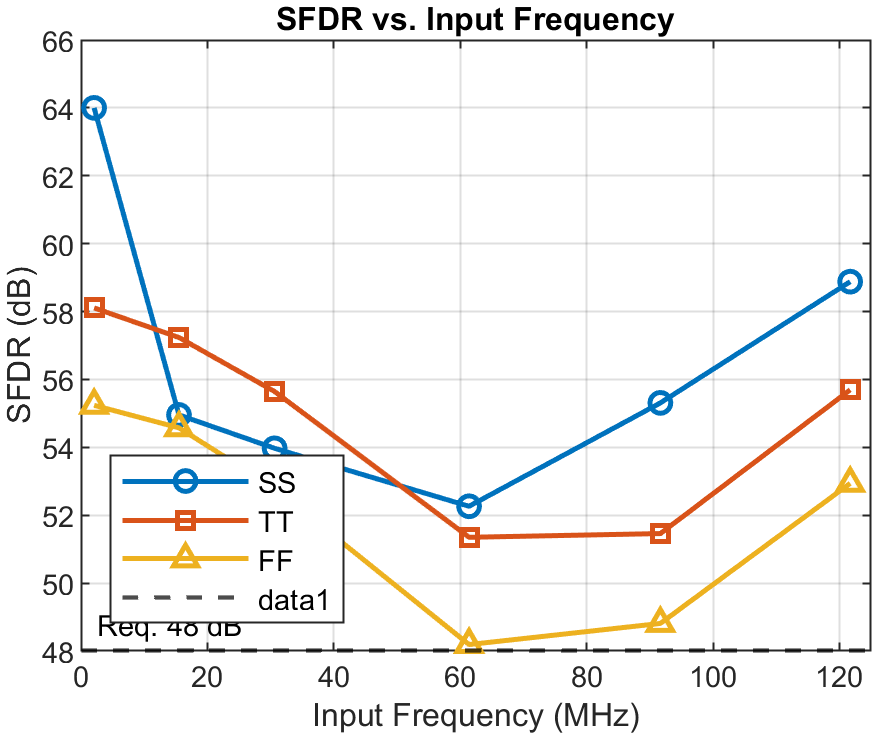
\includegraphics[width=\linewidth]{figures/Fig_SFDR_vs_freq.png}
    \caption{SFDR vs.\ input frequency across process corners.
             The dashed line marks the 48\,dB requirement.}
    \label{fig:sfdr_freq}
\end{figure}

\begin{figure}[H]
    \centering
    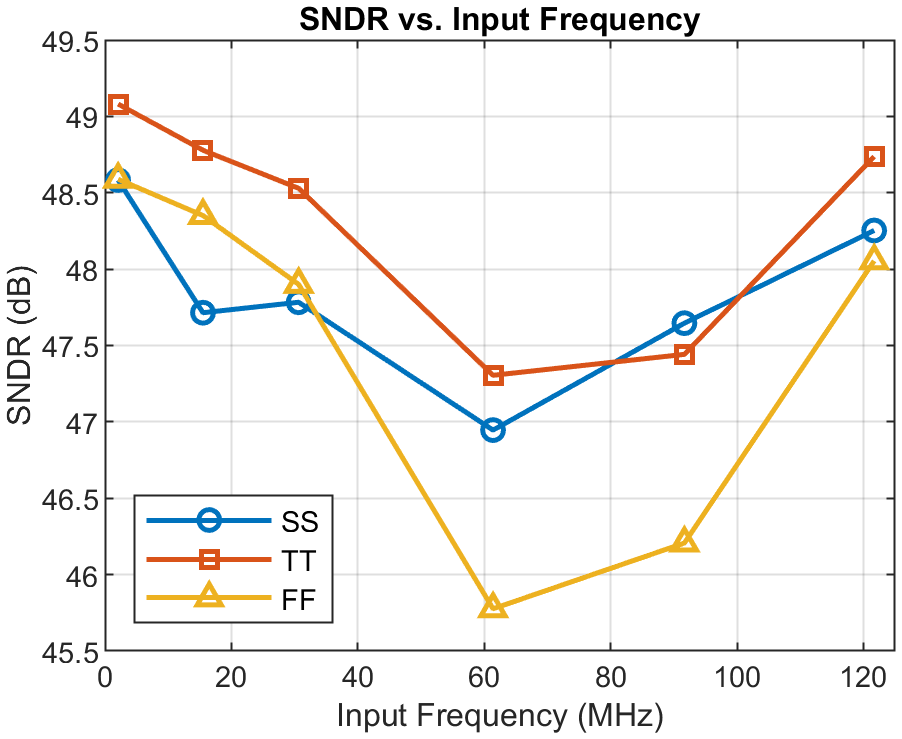
\includegraphics[width=\linewidth]{figures/Fig_SNDR_vs_freq.png}
    \caption{SNDR vs.\ input frequency across process corners.}
    \label{fig:sndr_freq}
\end{figure}

The TT corner achieves SFDR of 51–58\,dB and SNDR of 47–49\,dB across the
Nyquist band. The FF corner exhibits the worst SFDR, dropping to 48.2\,dB
at $f_\text{in} \approx 61$\,MHz — the minimum across all corners and frequencies,
which just meets the 48\,dB specification.
\subsection{Power Dissipation}
The power dissipation for each blocks are calculated separately by measuring their current drawn from Vdd source. 
\begin{gather}
    P = 1.8 \times I_{drawn} 
\end{gather}
For example, the bias generator continuously draw 100\textmu A from 1.8 V Vdd source. The power dissipation of it is
\begin{gather}
    P_\text{bias generator} = 100\mu \times1.8= 0.18mW
\end{gather}

For dynamic blocks such as input retimer, we average out its current over time, 
\begin{gather}
    P =1.8\times \text{avg}( I_\text{drawn})
\end{gather}
Power dissipation information are recorded in Table \ref{tab:perf}. 

\subsection{Performance Summary}

Table~\ref{tab:perf} summarizes the key simulated performance metrics.

\begin{table}[!h]
  \renewcommand{\arraystretch}{1.2}
  \caption{Performance Summary Across Process Corners}
  \label{tab:perf}
  \centering
  \begin{tabular}{lccc}
    \toprule
    \textbf{Parameter} & \textbf{SS} & \textbf{TT} & \textbf{FF} \\
    \midrule
    $V_\text{diff,pp}$ (V)                        & 1.501 & 1.502 & 1.501 \\
    $V_\text{CM}$ (V)                             & 1.424 & 1.423 & 1.423 \\
    \midrule
    DNL peak (LSB)                                & $-$0.172 & $-$0.026 & $-$0.012 \\
    INL peak (LSB)                                & $\pm$0.086 & $\pm$0.159 & $\pm$0.235 \\
    \midrule
    SFDR @ $f_\text{in}$\,=\,2.1\,MHz (dB)       & 64.0  & 58.1  & 55.2  \\
    SFDR @ $f_\text{in}$\,=\,121.7\,MHz (dB)     & 58.9  & 55.7  & 52.9  \\
    SFDR minimum across Nyquist (dB)              & 52.3  & 51.4  & 48.2  \\
    \midrule
    SNDR @ $f_\text{in}$\,=\,2.1\,MHz (dB)       & 48.6  & 49.1  & 48.6  \\
    SNDR @ $f_\text{in}$\,=\,121.7\,MHz (dB)     & 48.3  & 48.7  & 48.1  \\
    \midrule
    ENOB @ $f_\text{in}$\,=\,2.1\,MHz (bits)     & 7.78  & 7.86  & 7.78  \\
    ENOB @ $f_\text{in}$\,=\,121.7\,MHz (bits)   & 7.72  & 7.80  & 7.69  \\
    \midrule
    Trim tuning range (\%)                        & \multicolumn{3}{c}{$-14.8$ to $+14.3$} \\
    \midrule
    Power — Trim DAC     (mW)                & 0.2873 &  0.2908 & 0.2946 \\
    Power — Retimer \& Logic (mW)                & 16.16  & 18.66 & 23.31 \\
    Power — Bias Generator    (mW)                & 0.18 & 0.18 &  0.18\\
    Power — DAC Core         (mW)                & 27.03  & 28.08 & 28.9 \\
    \textbf{Total Power}      (mW)                & -- & -- & -- \\
    \bottomrule
  \end{tabular}
\end{table}

\subsection{SFDR Limiting Factors}

The primary SFDR bottleneck is the switching nonlinearity of the high-weight
current cells (MSB and MSB$-$1).
In a binary-weighted architecture, the MSB cell alone carries 128 LSBs of current
and uses 128 parallel switch transistors; the large gate capacitance of these
wide devices causes code-dependent charge injection and finite rise/fall time
at the switch drains, producing harmonic distortion.
The degradation is most pronounced in the FF corner because faster transistors
exhibit larger gate capacitance, steeper drain current transients, and greater
charge injection.
The minimum SFDR (48.2\,dB in FF at 61\,MHz) occurs at mid-frequency, where
the aliases of even-order switching transients from the MSB cells fall inside
the passband.
The NAND-latch retimer suppresses HD2 by ensuring $D_p$ and $D_n$ switch
symmetrically, but odd-order harmonics (HD3) remain, ultimately limiting SFDR.

% -----------------------------------------------------------------------
\section{Conclusion}
\label{sec:conc}

An 8-bit, 250\,MS/s binary-weighted current-steering DAC was designed in TSMC
0.18\,\textmu m CMOS.
The design meets all static specifications: differential output swing of
1.50\,V$_{\text{pp,diff}}$, DNL\,$<$\,0.18\,LSB, and INL\,$<$\,0.24\,LSB
across TT, SS, and FF corners.
The 6-bit analog weight trim DAC provides a $\pm$14\% tuning range per bit,
exceeding the $\pm$10\% requirement.
Dynamic performance satisfies the 48\,dB SFDR target across the Nyquist band
for all corners, with the tightest margin occurring in the FF corner at
mid-frequency inputs (48.2\,dB).
The dominant SFDR limiter is the switching nonlinearity of the MSB current cell,
driven by code-dependent charge injection in the wide switch transistors.
Power consumption data is pending and will be reported in the final submission.

% -----------------------------------------------------------------------
\end{document}
